\chapter[Anwendung: Variationelles Modell von LiFePO4 Akkumulatoren]{Anwendung: Variationelles Modell von LiFePO\(_4\) Akkumulatoren}{\label{ch:battery}}
Inspiration: \cite{Stinson_2021} \\
Lithium-Akkumulatoren haben in den letzten Jahrzehnten eine revolutionäre Veränderung in der Energiespeicherindustrie bewirkt. Diese wiederaufladbaren Batterien sind bekannt für ihre hohe Energiedichte, lange Lebensdauer und schnelle Ladezeiten, wodurch sie zu einer beliebten Wahl für eine Vielzahl von Anwendungen geworden sind. Lithium-Batterien basieren auf der Verwendung von Lithiumverbindungen als Elektrolyt und Elektrodenmaterialien, was zu einer effizienten und zuverlässigen Stromversorgung führt. Sie werden in Geräten wie Mobiltelefonen, Laptops, Elektrofahrzeugen und sogar in Energiespeichersystemen für erneuerbare Energien eingesetzt. Diese Batterien haben eine große Bedeutung für die Energiewende und tragen zur Reduzierung von Treibhausgasemissionen und der Abhängigkeit von fossilen Brennstoffen bei. Die kontinuierliche Forschung und Entwicklung im Bereich der Lithium-Batterien zielt darauf ab, ihre Leistungsfähigkeit weiter zu verbessern und gleichzeitig Kosten zu senken, um ihre Anwendbarkeit in verschiedenen Branchen zu erweitern.
\section{Physikalische Einführung}{\label{sec:phyintrobatt}}
\subsection[Aufbau von LiFePO4 Akkumulatoren]{Aufbau von LiFePO\(_4\) Akkumulatoren}{\label{subsec:strucbatt}}
Quelle für dieses Unterkapitel: \cite{LiAkkuSkillLync} \\
Lithium-Akkumulatoren bestehen in der Regel aus mehreren grundlegenden Komponenten, die zusammenarbeiten, um elektrische Energie zu speichern und abzugeben. Der grobe Aufbau liest sich wie folgt:
\begin{itemize}
    \item \textbf{Anode:} Die Anode ist die negative Elektrode der Batterie und besteht typischerweise aus Graphit (Graphit ist das (Stand September 2023) optimale Material bezüglich elektrischer Leitfähigkeitsmaximierung und gleichzeitiger Kostenminimierung) oder einem anderen kohlenstoffbasierten Material. Beim Entladen der Batterie gibt die Anode Lithium-Ionen ab.
    
    \item \textbf{Kathode:} Die Kathode ist die positive Elektrode der Batterie und besteht aus einer Verbindung, die Lithium-Ionen aufnimmt, wenn die Batterie aufgeladen wird. Die Kathode kann aus verschiedenen Materialien bestehen, wie beispielsweise Lithiumkobaltoxid (LiCoO\(_2\)), Lithiumeisenphosphat (LiFePO\(_4\)) oder Lithiumnickel-Mangan-Kobaltoxid (LiNiMnCoO\(_2\)) (wir werden - wie der Titel des Kapitels bereits suggeriert - im Folgenden den LiFePO\(_4\)-Fall betrachten).

    \item \textbf{Elektrolyt:} Der Elektrolyt ist eine leitfähige Substanz, die es Lithium-Ionen ermöglicht, zwischen der Anode und der Kathode zu wandern. In Lithium-Ionen-Batterien wird häufig ein organisches Lösungsmittel mit Lithiumsalzen als Elektrolyt verwendet. Es gibt auch feststoffbasierte Elektrolyte, die anstelle von flüssigen Elektrolyten eingesetzt werden können.

    \item \textbf{Separator:} Der Separator ist eine dünne poröse Membran, die zwischen der Anode und der Kathode platziert wird, um einen direkten Kontakt zwischen den beiden Elektroden zu verhindern und Kurzschlüsse zu vermeiden. Der Separator erlaubt jedoch den Durchtritt von Lithium-Ionen.

    \item \textbf{Gehäuse:} Das Gehäuse umgibt die internen Komponenten der Batterie und schützt sie vor äußeren Einflüssen. Es besteht in der Regel aus einem stabilen Metall oder Kunststoff.
\end{itemize}

\begin{figure}[label={fig:liakkuaufbau}, caption={Aufbau eines Lithium-Akkumulators \cite{LyncPicLi}}]
    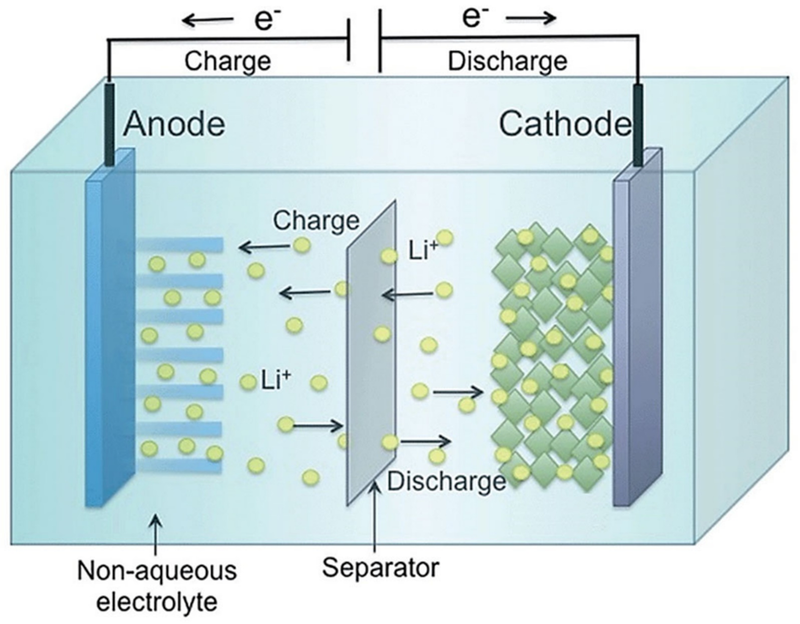
\includegraphics[scale=0.6]{figures/mceclip0_1642665078.png}
\end{figure}
\subsection{Beschreibung von Tensoren verschiedener Ordnungen in der Physik}{\label{subsec:tensorphy}}
Inspiration: \cite{NasaTensors} \\
Um einen Lithium-Akkumulator mathematisch erfassen zu können, werden wir aufgrund der auftretenden Elastizität auf die Theorie der Tensoren zurückgreifen müssen. Intuitiv gesprochen entspricht ein Tensor der Ordnung n einer "n-dimensionalen Matrix". Die Vorstellung von Matrizen in "hintereinanderliegenden" Ebenen ist deshalb eine gute erste Intuition. Dabei erinnern wir daran, dass wir für einen \((r,s)\)-Tensorraum mit \(r,s \in \mathbb{N}\), die Summe \(r+s =: n\) als Ordnung bezeichnen. Wir beschreiben nun Anwendungen aus der Physik:
\begin{itemize}
    \item \textbf{Tensoren der Ordnung 0 (Skalare):} Diese stellen lediglich eine einzelne Zahl dar. In der Physik wird er demnach verwendet, um Größen wie Masse, Temperatur oder Energie darzustellen.

    \item \textbf{Tensoren der Ordnung 1 (Vektoren):} Diese enthalten die Richtung und den Betrag einer physikalischen Größe. In der Physik werden diese zum Beispiel zur Darstellung von Geschwindigkeit und Kraft verwendet.

    \item \textbf{Tensoren der Ordnung 2:} Diese können durch eine Matrix repräsentiert werden. Beispielsweise wird der Spannungstensor in der Festkörpermechanik verwendet, um die Spannungsverteilung in einem deformierten Festkörper zu beschreiben. Der metrische Tensor in Einstein's allgemeiner Relativitätstheorie besitzt ebenfalls die Ordnung 2.

    \item \textbf{Tensoren der Ordnung 3:} Diese werden in der Kontinuumsmechanik verwendet, um komplexe Verformungs- und Spannungszustände zu beschreiben. In der Strömungsmechanik werden sie verwendet, um die turbulenten Eigenschaften von Strömungen zu analysieren.

    \item \textbf{Tensoren der Ordnung 4:} Diese werden in der Kontinuumsmechanik verwendet, um Elastizität zu beschreiben. Wir werden deshalb für die Modellierung des Lithium-Akkumulators auf diese Art von Tensor im Folgenden zurückgreifen. Eine weitere wichtige Anwendung finden diese in der Data Science, da diese "multilayer networks" beschreiben.
    
    \item \textbf{Tensoren höherer Ordnung:} Diese werden zum Beispiel in der Quantenmechanik verwendet, um die Wechselwirkungen zwischen mehreren Teilchen zu beschreiben.
\end{itemize}
%%%%%%%%%%%%%%%%%%%%%%%%%%%%%%%%%%%%%%%%%%%%%%%%%%%%%%%%%%%%%%%%%%%%%%%%%%%5
\section{Analytische Betrachtung von Akkumulatoren: Akkumulatoren nahe des Gleichgewichtszustandes}{\label{sec:anabatt}}
Bevor wir die mathematische Beschreibung dieses Problems präsentieren können, erinnern wir kurz an folgendes Resultat aus der linearen Algebra zurück:\\
Betrachte eine Matrix \(M \in \mathbb{R}^{n \times m}\). Dann kann man jede solche Matrix in ihren symmetrischen und anti-symmetrischen Anteil zerlegen, i.e. es gilt:
\begin{equation}
    M = \frac{M + M^T}{2} + \frac{M - M^T}{2}.
\end{equation}
Dabei sei angemerkt, dass diese Darstellung eindeutig ist. Im Folgenden werden wir den symmetrischen Anteil der Jakobi-Matrix benötigen. Wir setzen also in gängiger Notation fest:
\begin{equation}
    u: \Omega \to \mathbb{R}^n, \, e(u):= \frac{Du + (Du)^T}{2}.
\end{equation}
Wir werden in diesem Unterkapitel der Arbeit von K. Stinson aus dem Jahr 2021 in \cite{Stinson_2021} folgen, betrachten also im Folgenden den Spezialfall \(\Omega \subset \mathbb{R}^2\) (der Grund hiefür ist, dass zu dem Zeitpunkt der Forschung in dessen Dokument die Gültigkeit des \(\Gamma\)-Konvergenz Resultats von [\ref{theo4.20}, Satz 4.20] nur für Dimension 2 bekannt war; K. Stinson übertrug die dortig benutzte Beweismethode auf das Akkumulator Modell). Für das vorliegende konkrete Anwendungsbeispiel liegt das Doppelpotential \(W\) in folgender Form vor:
\begin{equation}
    \tilde{W}(y) := \omega y(1-y) + k_B T (y \, log(y) + (1-y) log(1-y)), \forall y \in [0,1],
\end{equation}
wobei \(k_B\) die Boltzmann-Konstante, \(T\) den Temperaturwert (in Kelvin) und \(\omega \in \mathbb{R}\) die Mischungsenthalpie (Enthalpie entspricht informell gesprochen dem Wärmeinhalt) beschreibt. Das zugehörige Energie-Funktional trägt dann folgende Darstellung:
\begin{equation}{\label{eq5.4}}
\begin{array}{l}
\mathcal{I}_{\epsilon} : W^{1,2}(\Omega,\mathbb{R}^2) \, \times \, W^{1,2}(\Omega,[0,1]) \to \mathbb{R} \cup \{\infty\}, \\
    \begin{cases} \mathcal{I}_{\epsilon} (u,c,\Omega) := \int_{\Omega} \frac{1}{\epsilon} W(c) + \epsilon |\nabla c|^2 + \frac{1}{\epsilon} \mathcal{C} (e(u) - c e_0) \, : \, (e(u) - c e_0))\,d\lambda^2(x), \text{ falls }(u,c) \in \mathcal{A} \\
    \infty, \text{ sonst,}
    \end{cases}
\end{array}
\end{equation}
wobei 
\begin{itemize}
    \item \(\mathcal{A} := W^{1,2}(\Omega,\mathbb{R}^2) \, \times \, W^{1,2}(\Omega,[0,1])\),
    \item \(e_0 \in \mathbb{R}^{2 \times 2}\) die "Gitterfehlanpassung" (Engl. "lattice misfit"),
    \item \(W(y) := \tilde{W}(y) - \min_{\alpha \in [0,1]} \tilde{W}(\alpha) \, \forall y \in [0,1]\),
    \item \(c : \Omega \to [0,1]\) die normalisierte Lithium-Ionen-Dichte,
    \item \(u : \Omega \to \mathbb{R}^2\) die Materialverformung (Engl. "material displacement"),
    \item \(\mathcal{C} : \mathbb{R}^{2 \times 2} \to \mathbb{R}^{2 \times 2}_{sym}\) einen symmetrisch, positiv definiten Stiffness-Tensor vierter Ordnung mit 
    \begin{equation}
        \mathcal{C}(z) \, : \, z > 0 \, \forall z \in \mathbb{R}^{2 \times 2}_{sym} \text{ mit } z \neq 0
    \end{equation}
    beschreiben.
\end{itemize}
Bevor wir uns wieder dem \(\Gamma\)-Konvergenzresultat zuwenden, stellt sich zunächst die Frage, ob wir für \eqref{eq5.4} dieses mal einen allgemeinen Minimierer erwarten können. Wir prüfen hierfür die Bedingungen der direkten Methode [\ref{theo2.8}, Satz 2.8] im schwachen Sinne nach:
\begin{enumerate}
    \item Da \(\mathcal{A}\) schwach abgeschlossen ist (\textit{Dafür erinnern wir an das wohlbekannte Resultat, dass für \(p \in ]1,\infty[\) \(L^p(\Omega,\mathbb{R}^m)\) gleichmäßig konvex ist. Betrachte dann (angepasste Version von \cite{marcellan2018weighted}[Theorem 4.2]):
    \begin{equation}
        T : W^{1,p}(\Omega,\mathbb{R}^m) \to L^p(\Omega,\mathbb{R}^m), T(u) := \{D^{\alpha}u\}_{|\alpha| \leq 1}.
    \end{equation}
    Dieser Operator ist eine (bezüglich der Norm-Topologie) abgeschlossene und isometrische Einbettung, woraus folgt, dass \(W^{1,p}(\Omega,\mathbb{R}^m)\) ebenfalls gleichmäßig konvex ist als (bezüglich der Norm-Topologie) abgeschlossener Unterraum von \(L^p(\Omega,\mathbb{R}^m)\), insofern \(|\alpha| \leq 1\) gilt. Nach dem Lemma von Mazur ist \(W^{1,p}(\Omega,\mathbb{R}^m)\) damit als konvexe Menge auch schwach abgeschlossen (aus diesem Argument wird auch klar, warum in Anwendungsdokumenten in der Variationsrechnung niemand diese Bedingung nachprüft).}), genügt es, dass wir die Koerzivität von \(\mathcal{I}_{\epsilon}\) nachprüfen. Ohne weitere Annahmen an den Integranden von \(\mathcal{I}_{\epsilon}\) ist offensichtlich \(\mathcal{I}_{\epsilon}\) im Allgemeinen nicht koerziv. Wir werden darauf in \ref{sec:regumini} genauer eingehen.
    \item Konvexität des Integranden können wir im Allgemeinen \textbf{nicht} erwarten, da mittels physikalischer Annahmen, die wir an \(W\) setzen, \(W\) nicht konvex sein kann (Physikalisch ist zu erwarten, dass \(W(R) = 0\) gilt für alle \(R \in SO(N)\) (da deformationsfrei) und \(W(S) = \infty\) für alle \(S\) mit \(det (S) = 0\) (da singuläre Komprimierung)). Überlegungen zur Polykonvexität sind aber durchaus valide; für optimale Bedingungen an den Integranden von \(\mathcal{I}_{\epsilon}\) ist es aber natürlich besser, gleich nach quasikonvexen Bedingungen zu suchen. Dies ist in der Theorie ein valider Weg, der in der Praxis allerdings sehr schwierig zu lösen ist. Wir werden deshalb in \ref{sec:regumini} einen Existenzbeweis mittels zugehöriger Euler-Lagrange Gleichungen aufführen.
\end{enumerate}
Vergleicht man die Situation mit der aus früheren Kapiteln, so wird klar, dass eigentlich nur interessant ist, wie wir den Tensor \(\mathcal{C}\) "kontrolliert" bekommen. Für die restlichen Details verweisen wir dann auf das Dokument \cite{Stinson_2021}. Wir treffen in diesem Rahmen folgende Annahmen:
\begin{itemize}
    \item (H1) \(\mathcal{C}(z) \, : \, z > 0 \, \forall z \in \mathbb{R}^{2 \times 2}_{sym} \text{ mit } z \neq 0\),
    \item (H2) \(det(e_0) \leq 0, \, e_0 \in \mathbb{R}^{2 \times 2}_{sym}\).
\end{itemize}
An dieser Stelle werden wir kurz verifizieren, dass (H2) natürlicherweise auftritt. Dazu halten wir fest, dass nach (H1):
\begin{equation}
    \mathcal{C}(\mathbb{R}^{2 \times 2}_{skew}) = \{0\}
\end{equation}
gilt. Nun erinnern wir an ein Resultat aus der linearen Algebra, das besagt, dass
\begin{equation}
    \forall F \in \mathbb{R}^{n \times n}_{sym} \, \forall G \in \mathbb{R}^{n \times n}_{skew} \, : \, <F,G>_{Fr} := tr(F^T G) = 0
\end{equation}
gilt.
Damit existiert die folgende eindeutige Zerlegung:
\begin{equation}
    e_0 = e^{sym}_0 + e^{skew}_0,
\end{equation}
woraus
\begin{equation}
    \mathcal{C}((e(u) - ce_0) \, : \, (e(u) - ce_0)) = \mathcal{C}(e(u) - ce^{sym}_0) \, : \, (e(u) - ce^{sym}_0)
\end{equation}
folgt. Wir erhalten:\\[0.5cm]
\pgfsetfillopacity{0.1}\colorbox{generalYellow}{\begin{minipage}{16cm}{\textcolor{black}{\pgfsetfillopacity{1}}{\label{prop5.1}}}
\textbf{Proposition 5.1 (\cite{Stinson_2021}[Proposition 2.2]):} Angenommen, es gilt (H1) und es existiert \(u \in C(\Omega,\mathbb{R}^2) \cap PC^1(\Omega,\mathbb{R}^2)\) nicht-affin, sowie \(e(u) \in \{A,B\}e_0\) mit \(0 < A < \frac{1}{2} < B < 1\). Dann gilt (H2) und es existiert für \(\nu \in \mathbb{S}^1\)
\begin{equation}
    \mathbb{S}_{\nu} := a \otimes \nu - (B-A)e_0 \, \in \mathbb{R}^{2 \times 2}_{skew}
\end{equation}
für \(a \in \mathbb{R}^2\).
\end{minipage}}

\textsc{Beweis:} Wir erinnern hier noch einmal, dass \(S(Du) = \bigcupdot_{i \in I} \mathbb{M}_i\) gilt, wobei \((\mathbb{M}_i, \mathcal{T}_{ecl})\) \(C^1\)-Mannigfaltigkeiten sind. Damit existierten \(T_q\mathbb{M}_i\) und wir berechnen die tangentiale Ableitung \(D_t u(q)\), wobei \(t \in [t] \in T_q \mathbb{M}_i\) (Erinnerung: Die Definition der Äquivalenzklasse ist unabhängig von der Kartenwahl und da alle \(\mathbb{M}_i\) in \(\mathbb{R}\) eingebettet sind, ist auch die Wahl des Repräsentanten nicht wichtig, da in diesem Fall \(T_q \mathbb{M}_i \simeq \mathbb{R}\) gilt):
\begin{equation}
    (A e_0 + S)t = D_t u(q) = (B e_0 + \tilde{S})t,
\end{equation}
wobei \(S, \tilde{S} \in \mathbb{R}^{2 \times 2}_{skew}\). Äquivalent kann man das auch als
\begin{equation}
    ((B-A)e_0 + \mathbb{S}_{\nu})t = 0
\end{equation}
auffassen, wobei 
\begin{equation}
    \mathbb{S}_{\nu} = \begin{pmatrix}
0 & s\\
-s & 0
\end{pmatrix}
= \tilde{S} - S \, \forall s \in [0,1].
\end{equation} 
Daraus folgt direkt:
\begin{equation}
    (B-A)e_0 + \mathbb{S}_{\nu} = a \otimes \nu \, \stackrel{e_0 \, sym.}{\Leftrightarrow} \, (B-A)^2 \, det(e_0) + s^2 = 0.
\end{equation}
Diese Gleichung hat nur Lösungen, falls (H2) gilt. \QEDB

\textbf{Bemerkung:} Zuletzt stellt sich natürlich die Frage, inwiefern die Annahme
\begin{equation}
    e(u) \in \{A,B\}e_0
\end{equation}
valide ist. Selbstverständlich ist das für viele in der Natur vorkommende Gebiete ein Ausschlusskriterium, jedoch ist ein endliches \(\Gamma\)-Konvergenz Resultat irgendwann auch nicht mehr zu erwarten. Und genau das verifizierten J. Ball und R. James auch in \cite{ball1987fine}.\\

Besagtes \(\Gamma\)-Konvergenz Resultat liest sich dann wie folgt:\\[0.5cm]
\pgfsetfillopacity{0.1}\colorbox{generalYellow}{\begin{minipage}{16cm}{\textcolor{black}{\pgfsetfillopacity{1}}{\label{theo5.2}}}
\textbf{Satz 5.2 (\cite{Stinson_2021}[Theorem 1.1]):} Sei \(\Omega \subset \mathbb{R}^2\) offen, beschränkt, strikt sternförmig mit Lipschitz-Rand. Angenommen (H1) und (H2) gelten. Dann gilt:
\begin{equation}
    \Gamma-\lim_{\epsilon \to 0^+} \mathcal{I}_{\epsilon} = \mathcal{I}_0 := \begin{cases}
        \sigma^* \mathcal{H}^{1} (S(Du) \cap \Omega), \text{ falls }c \in \mathcal{BV}(\Omega,\{A,B\}), \, u \in W^{1,2}(\Omega,\mathbb{R}^2), \, e(u) = c e_0 \\
        \infty, \text{ sonst,}
    \end{cases}
\end{equation}
wobei
\begin{equation}
\begin{array}{l}
    \sigma^* := \inf \{\liminf_{h \to \infty} \mathcal{I}_{\epsilon_h} (u_h,c_h,Q_{\nu}) \, | \epsilon_h \to 0, \\
    u_h \in W^{1,2}(Q_{\nu},\mathbb{R}^2), u_h \to \tilde{u}_{\nu} \text{ in }W^{1,2}(Q_{\nu},\mathbb{R}^2), \\
    c_h \in W^{1,2}(Q_{\nu},[0,1]), c_h \to \tilde{c}_{\nu} \text{ in }L^2(Q_{\nu})\}
\end{array}
\end{equation}
mit
\begin{itemize}
    \item \(\tilde{u}_{\nu}(x,y) := \begin{cases}
        Ae_0(x,y)^T, \text{ falls }(x,y) \cdot \nu < 0 \\
        (Be_0 + \mathbb{S}_{\nu})(x,y)^T, \text{ falls }(x,y) \cdot \nu > 0
    \end{cases}\),
    \item \(\tilde{c}_{\nu}(x,y) := \begin{cases}
        A, \text{ falls }(x,y) \cdot \nu < 0 \\
        B, \text{ falls }(x,y) \cdot \nu > 0
    \end{cases}\).
\end{itemize}
\end{minipage}}\\

\textbf{Bemerkung:} Dieses Resultat ist intuitiv exakt das, was wir nach all der Vorarbeit erwarten würden; vergleiche mit \eqref{eq4.60} und [\ref{prop5.1}, Proposition 5.1].\\

\textsc{Beweisskizze:} Das \(\Gamma\)-Liminf Resultat ist ein leicht modifiziertes Argument, wie wir es in \ref{sec:solsolphase} bereits gesehen haben. Wir fassen hier also nur die Ideen für das Kompaktheits- und \(\Gamma\)-Limsup Resultat zusammen:
\begin{itemize}
    \item \textbf{Kompaktheit (\cite{Stinson_2021}[Theorem 3.1.]):} Das Vorgehen ist das in der Existenztheorie von partiellen Differentialgleichungen übliche: Zunächst möchten wir Beschränktheit von \(u_h\) zeigen (das Kompaktheitsresultat für \(c_h\) erhält man analog wie im Modica-Mortula Theorem [\ref{theo4.3}, Satz 4.3]), die wir direkt aus der Koerzivität von \(\mathcal{C}\) und einer Anwendung von Korn's Ungleichung auf:
    \begin{equation}
        v_h (x,y) := u_h (x,y) - (\intbar_{\Omega} e(u_h(z)) \,d\lambda^2(z)) (x,y)^T + \alpha_h,
    \end{equation}
    wobei \(\alpha_h\) so gewählt, dass \(\int_{\Omega} v_h(z) \,d\lambda^2(z) = 0\) gilt. Es bietet sich hier Korn statt üblicherweise Gronwall an, da Korn's Ungleichung eine Verallgemeinerung von der Tatsache, dass der Gradient eines schief-symmetrischen Vektorfelds konstant gleich einer schief-symmetrischen Matrix ist, darstellt. Wir erhalten außerdem aus Koerzivität und Dreiecksungleichung, dass \(e(u) = ce_0\) gelten muss.
    \item \textbf{\(\Gamma\)-Limsup (\cite{Stinson_2021}[Theorem 6.1.]):} Wir suchen nun wie üblich nach "recovery sequences". Wir benötigen hier natürlich sowohl für \(u_h\), als auch für \(c_h\) jeweils eine solche Folge. Dabei erhalten wir die "recovery sequence" für \(c_h\) wieder direkt aus [\ref{theo4.3}, Satz 4.3], für \(u_h\) ist allerdings etwas Arbeit nötig. Dank der strikten Sternförmigkeit von \(\Omega\) erhalten wir wieder ein Problem mit \textbf{endlich} vielen Schnittstellen. Wir legen wieder Rechtecke um die Schnittstellen und zeigen auf einer definierten partiellen Ordnung für \(\Omega\) ohne die Schnittstellen, dass wir diese Rechtecke infitessimal klein wählen können, sodass wir am Ende die Eigenschaften der "optimal profile energy" wieder nutzen, um aus all diesen Informationen zusammengesetzt, schließlich unsere gesuchte "recovery sequence" zu erhalten. \QEDB
\end{itemize}
%%%%%%%%%%%%%%%%%%%%%%%%%%%%%%%%%%%%%%%%%%%%%%%%%%%%%%%%%%%%%%%%%%%%%%%%%
\section{Analytische Betrachtung von Akkumulatoren im Allgemeinzustand: Existenz und Regularität von Minimierern der Gesamtenergie}{\label{sec:regumini}}
Bisher haben wir uns reinen \(\Gamma\)-Konvergenz Resultaten gewidmet. Damit kennen wir das Verhalten, wenn wir uns einem Gleichgewichtszustand nähern. Wir haben aber bei Weitem noch nicht alle interessanten analytischen Fragen geklärt. Diese umfassen z.B.:
\begin{itemize}
    \item Wie sehen Minimierer von \(\mathcal{I}_{\epsilon}\) allgemein aus? Welche Regularität kann man erwarten?
    \item Existieren überhaupt schwache Lösungen?
    \item Falls ja, existieren dann auch klassische Lösungen? Wann ist ihr "Blow-Up"?
\end{itemize}
Wir wollen uns nun kurz mit diesen drei Punkten beschäftigen. Kurz deshalb, da eine tiefergehende Betrachtung den Umfang einer zweiten Masterarbeit annehmen würde. Wir ergänzen hierbei das Vorgehen von K. Stinson aus seiner Doktorarbeit \cite{stinson2021analysis}.\\

Wir sind also an expliziten Minimieren von \(\mathcal{I}_{\epsilon}\) interessiert. O.B.d.A. betrachten wir (sonst reskaliere das Funktional):
\begin{equation}
    \mathcal{I}(u,c,\Omega) := \int_{\Omega} W(c) + \frac{1}{2} |\nabla c|^2 + \frac{1}{2} \mathcal{C}(e(u) - ce_0) \, : \, (e(u) - ce_0) \,d\lambda^n(x)
\end{equation}
und berechnen die erste Variation bezüglich \(c\):
\begin{equation}
    \forall \phi \in C^{\infty}_c(\Omega,[0,1]) \, : \, \delta_c \mathcal{I}(c,\phi) = W'(c) - \Delta c + \mathcal{C}(ce_0 - e(u)) \, : \, e_0,
\end{equation}
natürlich vorausgesetzt, der Integrand ist passend majorisiert. Wir werden dies als eine der Annahmen mit aufführen im Folgenden.\\
Nun statten wir das Problem noch mit Robin-Randbedingungen aus, die wir hauptsächlich auf dem parabolischen Zylinder formulieren werden, i.e. auf:
\begin{equation}
    \Omega_T := \Omega \times ]0,T[, \, \Sigma_T := \Gamma \times ]0,T[, \, \Gamma := \partial \Omega \, \forall T > 0.
\end{equation}
All diese Vorüberlegungen führen dann auf das "Cahn-Hilliard reaction" Modell (CHR):
\begin{equation}{\label{eq5.22}}
    CHR \begin{cases}
        \partial_t c = \Delta \mu \text{ in }\Omega_T\\
        \mu = -\Delta c + W'(c) + \mathcal{C}(ce_0 - e(u)) \, : e_0 \text{ in }\Omega_T\\
        div(\mathcal{C}(e(u) - ce_0)) = 0 \text{ in }\Omega_T\\
        \partial_{\nu}c = 0 \text{ auf }\Sigma_T\\
        \partial_{\nu} \mu = R(c,\mu) \text{ auf }\Sigma_T\\
        \mathcal{C}(e(u) - ce_0)\nu = 0 \text{ auf }\Sigma_T\\
        c(0) = c_0 \text{ in }\Omega
    \end{cases},
\end{equation}
wobei \(R\) die Reaktionsrate beschreibt, definiert durch:
\begin{equation}
    R(c,\mu) := k_{ins}exp(C_1(C_2 - \mu)) - k_{ext}c exp(C_1(\mu - C_2)),
\end{equation}
wobei \(C_1, \, C_2, \, k_{ins}, \, k_{ext} > 0\) Konstanten sind. Hierbei beschreiben "\(ins\)" die Insertion und "\(ext\)" die Extraktion von Lithium-Ionen. In gewohnter Manier beweisen wir zunächst die Existenz schwacher Lösungen, um anschließend klassische Lösungen durch Regularitätsargumente zu erhalten. Dafür testen wir, integrieren dann partiell und halten fest, dass wir schwachen Lösungen folgender Form interessiert sind:\\[0.5cm]
\pgfsetfillopacity{0.1}\colorbox{generalYellow}{\begin{minipage}{16cm}{\textcolor{black}{\pgfsetfillopacity{1}}{\label{def5.3}}}
\textbf{Definition 5.3 (\cite{stinson2021analysis}[Definition 4.0.1]):} Eine schwache Lösung \((c,u)\) des CHR Modells erfüllt folgende Bedingungen für ein \(\delta > 0\):
\begin{enumerate}
    \item \(c \in L^{(2^\# - \delta)'}(0,T,W^{3,2}(\Omega)) \cap C([0,T[,L^2(\Omega))\),
    \item \(\partial_t c \in L^{(2^\# - \delta)'}(0,T,(W^{1,2}(\Omega))^*)\),
    \item \(u \in L^{(2^\# - \delta)'}(0,T,\dot{W}^{2,2}(\Omega,\mathbb{R}^N))\),
    \item \(c(0) = c_0 \in W^{1,2}(\Omega)\),
\end{enumerate}
sowie \(\lambda^1(t)\)-f.ü.:
\begin{equation}
\begin{array}{l}
     -<\partial_t c(t),\varphi> = \int_{\Omega} \nabla \mu(t) \cdot \nabla \varphi \,d\lambda^N(x) - \int_{\Gamma} R(c(t),\mu(t))\varphi \,d\mathcal{H}^{N-1}(x),\\
     \int_{\Omega} \mathcal{C}(e(u(t)) - c(t)e_0) \, : \, e(\psi) \,d\lambda^N(x) = 0
\end{array}
\end{equation}
für alle \(\varphi \in W^{1,2}(\Omega), \, \psi \in W^{1,2}(\Omega,\mathbb{R}^N)\). Hierbei ist \(\lambda^1(t)\)-f.ü. \(\mu(t) \in W^{1,2}(\Omega)\) definiert durch:
\begin{equation}
    <\mu(t),\varphi>_{L^2(\Omega)} := \int_{\Omega} \nabla c(t) \cdot \nabla \varphi + W'(c(t))\varphi + \mathcal{C}(c(t)e_0 - e(u(t))) \, : \, e_0 \varphi \,d\lambda^N(x).
\end{equation}
\end{minipage}}

\textbf{Bemerkung:} 
\begin{itemize}
    \item \(2^*\) beschreibt hier wie üblich den kritischen Sobolevexponenten. \(2^\#\) entspricht dem kritischen Spuroperatorexponenten, i.e. der Exponent, der nötig ist, damit der Spuroperator nach \(L^{2^\#}(\Gamma,\mathbb{R}^N)\) stetig ist. Genau genommen ist er definiert durch:
    \begin{equation}
        2^\# := \begin{cases}
            \frac{2N-2}{N-2}, \text{ falls }N>2 \\
            C, \text{ falls }N=2 \\
            \infty, \text{ falls }N=1
        \end{cases},
    \end{equation}
    wobei \(C > 0\) beliebig, aber fest.
    \item Das Apostroph in \((2^\# - \delta)'\) steht für den Hölder-konjugierten Exponenten.
    \item Die Räume in (1) - (3) sind Bochner-wertig, weshalb die Integrale als Bochner-Integrale zu verstehen sind. Damit ist die Notation des Lebesgue-Maßes als Lebesgue-Maß bezüglich dem "Limes von Treppenfunktionen" zu verstehen.
    \item \(\dot{W}^{2,2}(\mathbb{R}^N)\) bezeichnet die homogene Version von \(W^{2,2}(\mathbb{R}^N)\). Diese Homogenität ist zu verstehen als die Vervollständigung des Schwartz-Raumes \(\mathcal{S}(\mathbb{R}^N)\) bezüglich der Norm:
    \begin{equation}
        ||f||_{\dot{W}^{2,2}(\mathbb{R}^N)} := |||x|^2 \hat{f}||_{\mathbb{R}^N} \, \forall x \in \mathbb{R}^N,
    \end{equation}
    wobei \(\hat{f}\) die Fourier-Transformierte von \(f \in \mathcal{S}(\mathbb{R}^N)\) bezeichnet.
\end{itemize}
Für den folgenden Existenzbeweis nehmen wir dann an, dass gilt:
\begin{itemize}
    \item (H1) Es gilt \(|\mu(z_t)| \leq \Phi \in L^1(\Omega)\), wobei \(z_v := (t,c(t) + v\phi, \nabla c +  v \nabla \phi), \, \phi \in \mathcal{C}_c^{\infty}(\Omega)\).
    \item (H2) Für ein \(C > 0\) ist \(\mu \in C^2(\mathbb{R})\) mit:
    \begin{equation}
        (\mu \geq -C \, \land \, |\mu''(s)| \leq C(|s|^{\frac{2^*}{2}-1} + 1)) \forall s \in \mathbb{R}.
    \end{equation}
    \item (H3) Es existiert \(G \in C^1(\mathbb{R}^2)\) mit:
    \begin{equation}
        \partial_w G(s,w) = R(s,w) \, \forall s, \, w \in \mathbb{R}.
    \end{equation}
    \item (H4) \(\exists C > 0 \, : \, (R(s,w_2) - R(s,w_1))(w_2 - w_1) \leq -C|w_2 - w_1|^2 \, \forall s, \, w_1, \, w_2 \in \mathbb{R}\).
    \item (H5) \(\exists C > 0 \, \exists \delta > 0 \, : \, |R(s,w)| \leq C(|s|^{2^\# - \delta - 1} + |w|^{2^\# - \delta - 1} + 1) \, \forall s,w \in \mathbb{R}\).
    \item (H6) \(\exists C > 0 \, : \, |R(s,\pm 1)| \leq C \, \forall s \in \mathbb{R}\).
\end{itemize}
Das Theorem liest sich dann wie folgt:\\[0.5cm]
\pgfsetfillopacity{0.1}\colorbox{generalYellow}{\begin{minipage}{16cm}{\textcolor{black}{\pgfsetfillopacity{1}}{\label{theo5.4}}}
\textbf{Satz 5.4 (\cite{stinson2021analysis}[Theorem 4.0.4]):} Sei \(\Omega \subset \mathbb{R}^N\) ein offenes, beschränktes Gebiet mit \(C^3\)-Rand. Für ein \(T > 0\) existiert unter der Annahme von (H1) - (H6) eine schwache Lösung des CHR Modells in \(\Omega_T\).
\end{minipage}}

\textsc{Beweisskizze:} Wie in einem Existenzbeweis schwacher Lösungen in PDE üblich, teilt sich der Beweis in drei Schritte auf:
\begin{enumerate}
    \item Finde eine approximative Lösung des CHR Modells.
    \item Beweise Energieabschätzungen.
    \item Gehe zum Limes über.
\end{enumerate}
Wir skizzieren nun die groben Ideen für diese Schritte:
\begin{enumerate}
    \item Die grundlegende Idee hatten C. Kraus und A. Roggensack 2016 in \cite{kraus2016existence}. Sie bewiesen eine schwache Lösung für CHR Modell, allerdings unter Hinzunahme eines Viskositätsterms in \(\mu\), i.e. sie betrachteten:
    \begin{equation}
        \mu_{vis} := \mu_{CHR} + \eta \partial_t c,
    \end{equation}
    wobei \(\eta > 0\). C. Kraus und A. Roggensack zeigten eine (durch die implizite Euler-Methode, i.e. eine Stufe der Runge-Kutta-Methode) Zeit-diskretisierte Lösung in folgendem Vorgehen: Zunächst wießen Sie die Existenz einer solchen Lösung nach. Bevor wir das entscheidende Existenzresultat hierfür formulieren können, müssen wir noch ein paar Definitionen einführen:
    \begin{itemize}
        \item Sei \(\mathcal{L} : L^{2^\# - \delta}(\Gamma, \mathbb{R}^N) \times L^2(\Omega,\mathbb{R}^N) \to \mathbb{R} \cup \{\infty\}\) ein Funktional definiert durch:
        \begin{equation}
            \mathcal{L}(c,v) := \begin{cases}
                \frac{1}{2} ||Dv||_{L^2(\Omega)}^2 - \int_{\Gamma} G(c,v) \,d\mathcal{H}^{N-1}(x), \text{ falls }v \in W^{1,2}(\Omega) \\
                \infty, \text{ sonst}
            \end{cases}.
        \end{equation}
        Es ist eigentlich, unterhalbstetig und dank (H5) auch konvex bezüglich \(v\) ((H5) garantiert auch die Wohldefiniertheit, da das Randintegral von \(G\) so endlich ist.). Im Folgenden beschreibt \(\mathcal{L}^*\) dann die Fenchel-Konjugierte zu \(\mathcal{L}\) bezüglich \(v\).
        \item Sei \(\mathcal{B} : L^{2^\# - \delta} (\Gamma,\mathbb{R}^N) \times W^{1,2}(\Omega,\mathbb{R}^N) \to (W^{1,2}(\Omega,\mathbb{R}^N))^*\) ein Operator definiert durch:
        \begin{equation}
            <\mathcal{B}(c,u),v> := \int_{\Omega} Du \, : \, Dv \,d\lambda^N(x) - \int_{\Gamma} R(c,u) \cdot v \,d\mathcal{H}^{N-1}(x).
        \end{equation}
        Fixieren wir \(c\) (wir schreiben dann \(\mathcal{B}_c(u)\)), so ist \(\mathcal{B}\) strikt monoton (nach (H4)), beschränkt (nach (H5)) und \(L^2\)-koerziv (nach (H4) (getestet mit \(w_2 = 1, \, w_1 = 0\)), (H5) und den Ungleichungen von Young und Poincare). Damit existiert (siehe [\ref{theoA.8}, Anhang A.8]; die Voraussetzung der radialen Stetigkeit ist erfüllt, da \(\mathcal{B}\) sogar stetig ist dank (H5)) der inverse Operator \(\mathcal{B}^{-1}: L^{2^\# - \delta} (\Gamma,\mathbb{R}^N) \times (W^{1,2}(\Omega,\mathbb{R}^N))^* \to W^{1,2}(\Omega,\mathbb{R}^N)\). Nach [\ref{theoA.8}, Anhang A.8] ist \(\mathcal{B}^{-1}\) zusätzlich strikt monoton, beschränkt und demistetig; sogar stetig, siehe \cite{kraus2016existence}[Lemma 1] (folgt hauptsächlich aus Minty's Trick).
    \end{itemize}
    Die Idee ist nun, das CHR Modell in der Zeit zu diskretisieren. C. Kraus, A. Roggensack und auch K. Stinson in \cite{stinson2021analysis} benutzten hierfür jeweils die implizite Euler-Methode. Fixiere also \(T > 0\) und betrachte als Zeit-Schritt \(\tau := \frac{T}{M}\) für ein \(M \in \mathbb{N}\). C. Kraus und A. Roggensack wießen in \cite{kraus2016existence}[Lemma 7] die entscheidende Existenz eines Minimiers des diskretisierten Energiefunktionals
    \begin{equation}
        \mathcal{I}_M^m(u,c,\Omega) := \mathcal{I}(u,c,\Omega) + \tau \mathcal{L}^*_{c_M^{m-1}}(-\frac{c - c_M^{m-1}}{\tau}), \, m=0,...,M-1
    \end{equation}
    nach (die Unterhalbstetigkeit für die direkte Methode folgt direkt aus der Unterhalbstetigkeit der Fenchel-Konjugierten; die \(L^2\)-Koerzivität ist eine kurze Rechnung mit den Ungleichungen von Poincare und Korn). Dieses Energiefunktional ist natürlich nicht willkürlich gewählt, sondern resultiert aus den Randbedingungen, die wir an das CHR Modell gestellt haben, hauptsächlich die Neumann-Randbedingung an \(\mu\) auf \(\Sigma_T\), siehe anschließende Bemerkung. Als logischen zweiten Schritt haben C. Kraus und A. Roggensack gezeigt, wie die zugehörigen diskretisierten Euler-Lagrange-Gleichungen aussehen, die der Minimierer erfüllt.
    \item Für die Interpolationsfunktionen:
    \begin{itemize}
        \item \(c_{\tau}(t) := \begin{cases}
            c_{\tau}^0, \text{ falls }t=0 \\
            c_{\tau}^{m+1}, \text{ falls }t \in ]m\tau,(m+1)\tau]
        \end{cases}\),
        \item \(c_{\tau}^-(t) := c_{\tau}^m, \text{ falls }t \in [m\tau,(m+1)\tau[\),
        \item \(\hat{c}_{\tau}(t) := \frac{(m+1)\tau - t}{\tau} c_{\tau}^m + \frac{t-m\tau}{\tau}c_{\tau}^{m+1}, \text{ falls }t \in [m\tau,(m+1)\tau[\)
    \end{itemize}
    findet man die folgenden Energieabschätzungen:\\[0.5cm]
    \pgfsetfillopacity{0.1}\colorbox{generalYellow}{\begin{minipage}{14cm}{\textcolor{black}{\pgfsetfillopacity{1}}{\label{lem5.5}}}
\textbf{Lemma 5.5 (\cite{stinson2021analysis}[Lemma 4.2.5]):} Sei \(\Omega \subset \mathbb{R}^N\) ein offenes, beschränktes Gebiet mit \(C^3\)-Rand. Unter den Annahme von (H1) - (H6) gelten folgende \textbf{gleichmäßigen} Energieabschätzungen:
\begin{equation}
\begin{array}{l}
    ||c_{\tau}||_{L^{\infty}(0,T,W^{1,2}(\Omega)} \leq C \\
    ||\partial_t \hat{c}_{\tau}||_{L^{(2^\# - \delta)'}(0,T,(W^{1,2}(\Omega))^*} \leq C \\
    ||\mu_{\tau}||_{L^{(2^\# - \delta)'}(0,T,W^{1,2}(\Omega)} \leq C \\
    ||c_{\tau}||_{L^{(2^\# - \delta)'}(0,T,W^{3,2}(\Omega)} \leq C,
\end{array}
\end{equation}
wobei \(\mu_{\tau}^m := \mathcal{B}^{-1}(c_{\tau}^{m-1},-\frac{c_{\tau}^m - c_{\tau}^{m-1}}{\tau})\).
\end{minipage}}
Hier wird nun entscheidend, dass wir mit \(2^\#\) den kritischen Exponenten für den Spuroperator gewählt haben, da wir mithilfe der ersten Energieabschätzung und eben der Stetigkeit des Spuroperators \(c_{\tau} \in L^{\infty}(0,T,L^{2^\# - \delta}(\Gamma))\) erhalten.
    \item In diesem Schritt wird klar, warum C. Kraus und A. Roggensack den zusätzlichen Viskositätsterm benötigt haben. Dieser Term erschloss Ihnen direkt die benötigte Regularität, um zu einer stetigen Lösung übergehen zu können (dabei mussten sie natürlich ein leicht modifiziertes Energiefunktional \(\mathcal{I}_M^m(u,c,\Omega)\) verwenden aufgrund des zusätzlichen Terms). Ohne diesen Term gilt es, ein Kompaktheitsresultat zu beweisen. In diesem Fall bietet sich die Strategie wie im Kompaktheitsresultat von Aubin-Lions-Simon (siehe [\ref{theoA.9}, Anhang A.9]) an. \QEDB
\end{enumerate}
\textbf{Bemerkung:} Wir sind noch eine Antwort schuldig, wie \(\mathcal{I}_M^m(u,c,\Omega)\) und das CHR Modell zusammenhängen. Dafür zeigen wir:
\begin{equation}
    (v^* \in \partial \mathcal{L}_c(v) \, \Leftrightarrow \, <v^*,\xi>_{L^2(\Omega)} = <B(c,v),\xi>_{W^{1,2}(\Omega)}) \, \forall \xi \in W^{1,2}(\Omega),
\end{equation}
wobei \(\partial\) hier das Subdifferential (für eine Definition siehe \eqref{eq.2.31}) bezeichnet. Für \(\mathcal{L}_c(v) < \infty\) ist \(\mathcal{L}_c(v)\) eigentlich, \textbf{konvex} und unterhalbstetig, also erhalten wir:
\begin{itemize}
    \item "\(\Leftarrow\)": Folgt direkt aus (H3), (H5) und der Young-Ungleichung;
    \item "\(\Rightarrow\)": Da \(\mathcal{L}_c(v)\) konvex ist, existiert \(\partial_w^+ \mathcal{L}_c(v)\) nach \cite{phelps2009convex}[Lemma 1.2.]. Nach Annahme ist \(v^* \in \partial \mathcal{L}_c(v)\), weshalb \(\mathcal{L}_c(v)\) Gateaux differenzierbar (i.e. \(\partial_w \mathcal{L}_c(v)\) existiert) nach \cite{phelps2009convex}[Proposition 1.8.] ist. Wir berechnen diese Gateaux-Ableitung und erhalten:
    \begin{equation}
        <v^*,w>_{L^2(\Omega)} = \partial_w \mathcal{L}_c(v) = <\mathcal{B}_c(v),w>.
    \end{equation}
\end{itemize}
Damit ist
\begin{equation}
    -\partial_t c \in \partial \mathcal{L}_c(\mu)
\end{equation}
und die Formulierung ist damit äquivalent zu dem CHR Modell. Diese äquivalente Umformulierung ist notwendig, um mithilfe von konvexer Dualitätstheorie variationelle Methoden anwenden zu können. C. Kraus und A. Roggensack zeigten den genauen Zusammenhang in \cite{kraus2016existence}[Seite 7 ff.] wie folgt:
\begin{equation}
    \partial \mathcal{L}_c^*(v^*) = \{\mathcal{B}_c^{-1}(v^*)\},
\end{equation}
also gilt insbesondere:
\begin{equation}
    \mu = \mathcal{B}_c^{-1}(-\partial_t c).
\end{equation}

Schließlich wollen wir das CHR Modell noch auf mögliche klassische Lösungen untersuchen. Nun ist das Modell nicht-linear, eine allzu lange Existenz klassischer Lösungen ist also nicht wirklich zu erwarten; üblicherweise tritt ein "Blow-Up" in solchen Fällen sehr schnell ein. Im Gegensatz zum schwachen Resultatstheorem werden wir hier aber sogar auf die Beweisskizze verzichten, da diese eine Einführung in sehr erweiterte Regularitätstechniken benötigen würden, wie "Bootstrap"-Methoden und spezielle Fixpunktsätze, wie der Fixpunktsatz von Schauder, eine Verallgemeinerung für topologische Vektorräume des bekannten Brouwerschen Fixpunktsatzes. K. Stinson bewies in \cite{stinson2021analysis} ein Regularitätsresultat nur für den nicht-eliptischen Fall, i.e. für:
\begin{equation}
    CHR_{nel} \begin{cases}
        \partial_t c = \Delta \mu, \text{ in }\Omega_T \\
        \mu = - \Delta c + W'(c), \text{ in }\Omega_T \\
        \partial_{\nu} c = 0, \text{ auf }\Sigma_T \\
        \partial_{\nu} \mu = R(c,\mu), \text{ auf }\Sigma_T \\
        c(0) = c_0, \text{ in }\Omega
    \end{cases}.
\end{equation}
Das Resultat liest sich wie folgt:\\[0.5cm]
\pgfsetfillopacity{0.1}\colorbox{generalYellow}{\begin{minipage}{16cm}{\textcolor{black}{\pgfsetfillopacity{1}}{\label{theo5.6}}}
\textbf{Satz 5.6 (\cite{stinson2021analysis}[Theorem 5.0.1]):} Sei \(\Omega \subset \mathbb{R}^3\) eine offene, beschränkte Menge mit glattem Rand, \(c_0 \in W^{4,2}(\Omega)\) mit:
\begin{equation}
    \epsilon < c_0(x) < 1 - \epsilon \text{ f.}\lambda^3-\text{f.a. }x \in \Omega,
\end{equation}
sowie \(\partial_{\nu} c_0 = 0, \, \partial_{\nu}(\Delta c_0) = -R(c_0,-\Delta c_0 + W'(c_0))\) auf \(\Gamma\). Dann existiert ein \(T = T(c_0) > 0\) und \(c \in W^{6,3/2}(\Omega_T)\), sodass \(c\) eine Lösung des \(CHR_{nel}\) Modells ist.
\end{minipage}}

\textbf{Bemerkung:} Da wir nach Morrey wissen, dass \(W^{6,3/2}(\Omega_T)\) in \(C^{3,\alpha}(\Omega_T)\) für alle \(\alpha \in ]0,1[\) einbettet, ist damit die Lösung \(c \in C^{3,\alpha}(\Omega_T)\).
%%%%%%%%%%%%%%%%%%%%%%%%%%%%%%%%%%%%%%%%%%%%%%%%%%%%%%%%%%%%%%%%%%%%%%%%%%%%%%%%%%%%%%%%%
\section[Verallgemeinerung in N Dimensionen: Geometrische Probleme]{Verallgemeinerung in \(\mathbb{N}\) Dimensionen: Geometrische Probleme}{\label{sec:gendim}}
Wir haben nun das \(\Gamma\)-Konvergenz und ein Regularitätsresultat für die Existenz von Lösungen bezüglich \eqref{eq5.4} gesehen. Wie bereits dort erwähnt, war zum Zeitpunkt der Forschung für die Arbeit von K. Stinson \cite{stinson2021analysis} nur das zugrundeliegende Modell für Dimension 2 bekannt. In \ref{subsec:soninva} haben wir am Ende in Schritt 2 gesehen, dass inzwischen ein Resultat für Dimension N von E. Davoli und M. Friedrich in \cite{davoli2020two} vorliegt - wenn auch unter der Hinzunahme eines zusätzlichen Stabilitätstermes. Lässt sich hier eine grundlegende allgemeine Beweisstrategie finden, so könnte man diese Strategie dann mit sehr hoher Wahrscheinlichkeit auch für das \(\Gamma\)-Konvergenz Resulat des Akkumulator-Modells in Dimension N nutzen.\\
Doch warum ist diese Verallgemeinerung derart kompliziert? Die Beweisstrategie von Conti und Schweizer in \cite{ContiSchweizerSolidSolid} baute \textbf{sehr} stark auf einem Starrheitsresultat für einzelne Segmente von \(\Omega\) \cite{ContiSchweizerSolidSolid}[Proposition 2.2] auf. Sie zeigten die "Erhaltung" der meisten Segmente nach Rotation (genauer gesprochen zeigten Sie, dass die zu den "erhaltenen" Segmenten komplementäre Menge kleines Maß und kleinen Perimeter besitzt.). Damit erhält man das gewünschte Endresultat durch Integration mit dem passenden Kurvenintegral.\\
Das große Problem an diesem Beweis ist, dass der Beweis entscheidend von Linien als Segmenten ausgeht und damit das Argument äußerst stark an die Dimension von \(\Omega\) bindet.\\
\section{Neue Ideen für das offene Dimensionsproblem}{\label{sec:newidea}}
Wir erinnern noch einmal daran, dass wir \eqref{eq4.138} zeigen wollen, i.e.
\begin{equation}
    \exists R \in SO(n) \, : \, ||Du - R \mathcal{M}||_{L^2(\Omega)} \leq C \epsilon.
\end{equation}
Ein starkes Werkzeug für Regularitätsprobleme aus der Theorie der PDE liefert die bekannte De Giorgi-Nash Theorie, entstanden in \cite{de1957sulla} bzw. \cite{nash1958continuity} und von Ladyzhenskaya und Ural'tseva in \cite{ladyzhenskaya1968linear} verallgemeinert zu den De Giorgi-Klassen. Diese Theorie wurde für quasi-lineare elliptische und parabolische PDE entwickelt. Nun betrachten wir allerdings ein \(SO(n)\)-invariantes Problem; auf einen quasi-linear elliptischen Rahmen sich einzuschränken ergibt also keinen Sinn. Es erscheint auch wenig sinnvoll, zu versuchen, die De Giorgi-Nash Theorie zu verallgemeinern, da bei solch allgemeiner Betrachtung überhaupt nicht klar ist, ob wir dann auch die Ordnung \(\epsilon\) erwarten können.\\
Eine widerrum vielversprechende Idee könnte eine Verknüpfung von Funktionalanalysis und Gruppentheorie sein. 